\chapterimage{chapter_head_2.pdf} % Chapter heading image

\chapter{Softwares no Ensino da Matemática}

\section{Introdução}\index{Introdução}

\indent Não pode ser desconsiderado a presença dos computadores no cotidiano das pessoas e esse processo não para mais, ou seja, a cada dia que passa a humanidade fica mais dependente dos computadores e, de modo mais genérico, da Tecnologia!

O conceito de Tecnologia em um primeiro momento, para a maior parte das pessoas, está relacionado com os computadores, mas isso não é verdade. \textbf{Tecnologia} pode ser entendido como \textit{o estudo da técnica}\footnote{O leitor pode pesquisar mais sobre a origem da palavra em outras fontes pois o objetivo neste material não é tratar sobre tal assunto.}.

Desse modo, é possível imaginar que o processo de preparar uma receita de um determinado bolo é fruto de uma \textit{tecnologia}, pois se alguém for repeti-la, a garantia de sucesso é grande. Um ponto que deve ficar claro é que "quem repete a receita" NÃO está criando tecnologia, está executando um processo, apenas.

No entanto, se alguma pessoa mais experiente, desenvolve um método diferenciado para a confecção de um bolo e consegue reprodutibilidade, pode-se imaginar que ela desenvolveu uma nova tecnologia para o preparo de bolo.

Essa discussão parece ser bem abstrata, porém o próximo passo auxiliará no entendimento do conceito.

É comum as pessoas pensarem que para \textit{haver tecnologia} DEVE ter a presença de máquinas (mecânicas, elétricas, etc) e isso não é verdade, as máquinas são frutos de uma tecnologia, ou seja, um determinado processo quando é bem estudado/conhecido pode ser reproduzido inúmeras vezes que sempre sairá do mesmo modo, assim as máquinas são criadas para garantir maior velocidade (não pode ser esquecido que alguém quer lucrar muito!), padronização gerando maior qualidade no processo e no bem manufaturado (serve, também, para serviços prestados).

Esse conceito apreendido permite entender os \textit{motivos} de fracasso quando se utiliza \textbf{recursos} computacionais no ensino. A maior parte dos "fracassos" está relacionada a má utilização/diferenciação dos conceitos sobre \textit{tecnologia} e \textit{recursos}.

Seguindo o raciocínio, \textit{recursos} são ferramentas/materiais disponíveis que pode ser utilizados num processo de escolarização, por exemplo. Assim, quando um professor de matemática leva seus alunos ao laboratório de informática da escola, ele DEVE ter em mente a discussão abordada anteriormente para que essa \textit{aula no laboratório} não seja encarada apenas como \textit{diversão} ou \textit{passatempo}; deve haver \textit{SENTIDO} no processo. O fato de estar no laboratório de informática não implica aprendizado efetivo diferenciado sempre. Para que a \textit{condicional}\footnote{O leitor que já estudou \textit{Lógica Matemática} já deve estar familiarizado com isso: $p \rightarrow q$} seja verdadeira as proposições devem ser verdadeiras, ou seja, sempre que for ao laboratório de informática (uso de celular, tablets em sala) deve garantir que exista aprendizado efetivo e, para isso, o professor deve, no mínimo, entender duas coisas: o recurso que está usando como suporte e os conceitos matemáticos que ele quer abordar na aula.

Esse ponto é complicado pois nenhum humano sabe tudo, e os sábios sabem disso porém, as aulas com a utilização de recursos computacionais acaba sendo uma via de mão dupla no aprendizado: o professor e o aluno aprendem. Isso também é conhecido como \textit{professor mediador, facilitador}.

Bom, entendido esta visão, resta um outro item: \textit{Como fazer a matemática ser interessante de tal modo que os recursos computacionais sejam usados, com prazer, permitindo resolver problemas do cotidiano do aluno?}

Uma parte será possível abordar aqui: resolução de problemas. A resolução de problemas não é algo tão simples de ser elaborado pelo profissional da educação pois deverá ter \textit{valor agregado} para fazer \textit{sentido} na vida do aluno. Deve, ainda, esquecer que \textit{existe linearidade no ensino de matemática}, ou seja, para aprender B, deve-se conhecer inicialmente A\footnote{Isso dá trabalho, gera intrigas, mas é gratificante!}.

A segunda parte, que é o foco principal para obter uma sociedade crítica e alfabetizada (de fato, não somente de direito!) é que o aluno consiga resolver seus problemas cotidianos. Mas quais problemas? Que tipos de problemas? Essas perguntas são difíceis e, portanto, o segundo item se encerrará aqui e ficando a critério e criatividade do leitor para desenvolver estratégicas transformadoras na vida das pessoas.

Enfim, não existe apenas uma interpretação e a visão abordada aqui é a visão particular do autor, não é uma verdade absoluta, mas deve servir para instigar a pensar de modo diferenciado.

\section{Determinação experimental do número $\pi$}\index{Determinação experimental do número $\pi$}

Será mostrado a seguir a utilização da \textit{tecnologia} para determinar, de modo aproximado, o valor numérico para a constante $\pi$. A \textit{metodologia} utilizada pode ser aplicada para qualquer nível de escolarização, ou seja, desde o sexto ano (prefiro quinta série!) até em pós-graduações. Deve ficar claro que a diferenciação deve estar no vocabulário usado em cada série. É claro que os níveis mais elevados possuam conhecimentos matemáticos mais sofisticados e os indivíduos desse nível possuem mais experiências e conceitos apreendidos ao longo da vida acadêmica.

Inicialmente, deve-se ter um problema instigante: \textit{Determinar a constante $\pi$ usando uma balança}.

O segundo passo consiste em um \textit{brainstorming} para tentar definir uma estratégia para a solução desse problema. Com a estratégia definida, o terceiro passo será a tentativa de resolução. Após a possível solução, deve-se testar em outros problemas semelhantes para verificar a validade do modelo e, se tudo estiver OK, problema resolvido. É possível a qualquer momento refazer o experimento com possíveis melhorias no processo não previstas anteriormente e testar novamente para ver se os resultados melhoram.

O \textit{brainstorming} mencionado não acontecerá aqui mas pode aplicado em uma sala de aula de modo que os participanetes (alunos) sugiram, sem medo de errar (no \textit{brainstorming} não existe ideias tolas ou imbecis) e o professor ficar anotando as ideias durante o tempo necessário até que as ideias se esgotem. Lembre-se: nada deve ser imposto, mas o convite deve ser irrecusável! Após o esgotamento das ideias, o professor deve começar a analisar as ideias em função de \textit{chance de sucesso para resolver o problema} explicando os conceitos, os prós e os contras de cada ideia. Isso motiva o pensamento crítico de qualquer humano engajado no problema.

Para resolver o problema proposto será necessário uma balança. Balanças, geralmente permitem medir a \textbf{massa} de um objeto e \textbf{NÃO} o \textbf{peso}, pois peso, de acordo com \textit{Newton} pode ser definido matematicamente como $\vec{P} = m \cdot \vec{g}$. Somente nessa visão já é possível explorar conceitos de um bimestre do ensino médio onde é falado sobre as leis de Newton, é possível falar sobre o planeta Terra (multidisciplinaridade, oi?), entre outros.

O exemplo de que isso pode explorado em todos os níveis, e linguagens, vem da relação mencionada sobre a diferença entre \textit{massa} e \textit{peso}:

\begin{ceqn}
	\begin{align*}
		\vec{P} = m \cdot \vec{g}
	\end{align*}
\end{ceqn}
	
	
O leitor pode ter lido a relação acima e ter pensado: \textit{Não foi assim que aprendi na escola! Não tinha essas setinhas em cima do P e do g}. Calma, até alunos de níveis elevadíssimos não sabem o motivo dessas setinhas em cima do $g$.

Lembrando: Força pode ser escrito como a multipliacação entre a massa e uma aceleração, matematicamente $F=m \cdot a$. Após ter lembrado sobre isso, o leitor pode ter imaginado sobre os \textit{diagramas de corpo isolado} em que as \textit{trações} e \textit{forças} são \textit{grandezas vetorias}, pois \textit{vetor} tem \textit{direção, sentido e módulo}. Mas se a Força é um vetor qual das duas grandezes que estão multiplicando é vetorial? Mas por que alguma dessas outras grandezas tem de ser vetorial? O que é um vetor? Etc.

Bom, a \textit{massa} de um corpo não depende se está indo para do Sul para o Norte ou da esquerda para a direita, a massa representa a quantidade de matéria de um objeto assim, massa não é vetorial é uma \textit{grandeza escalar}, basicamente, um número. Com esse raciocínio, a \textit{grandeza vetorial} só pode ser a aceleração que num \textit{sistema de coordenadas} representa uma \textit{direção e sentido} e possui uma \textit{intensidade} ou \textit{módulo}. O mesmo acontece com a força \textit{Peso}; a massa é \textit{escalar} então a aceleração \textit{gravitacional} só pode ser \textit{vetorial}, incrível! O leitor pode imaginar o motivo de todo o tempo sempre usar a aceleração gravitacional apenas $g$ e não $\vec{g}$. Isso é possível? A resposta é: SIM, totalmente! Por quê? Pois nesses estudos apenas o valor da aceleração, ou seja, o \textit{módulo} é fundamental porém, em outras situações, a aceleração gravitacional deve ser pensado como uma grandeza vetorial pois as flutuações do campo gravitacional existem e isso pode influenciar, por exemplo, o funcionamento de um satélite.

Ainda não foi separado os materiais ou alguma metodologia para determinar a constante $pi$ e já foi possível abordar muitos conceitos relacionados (multidisciplinaridade, oi?).

Voltando ao problema, deve-se pensar que a determinação da constante $pi$ através do uso de uma balança está intimamente ligado com o volume de algo e, novamente, conceitos adicionais aparecem para serem estudados: ponto, linha, área e volume. Isso está relacionado a \textit{dimensões} e a expansão de alguns axiomas. O ponto não tem dimensão, dois pontos formam uma reta (linha - 1D, comprimento), uma figura plana possui duas dimensões (2D, comprimento e largura) e um sólido possui três dimensões (3D, comprimento, largura e altura). O leitor deve pensar que nada na vida real possui apenas duas dimensões ou uma dimensão; por mais que se tente representar uma linha através de um lápis e régua, a espessura do grafite deixada numa folha torna essa linha um objeto 2D, expandindo mais, o grafite deixado na folha formou um sulco com o depósito de material (grafite) tornando assim um objeto 3D! (multidisciplinarida, oi?) Os objetos perfeitos encontram-se apenas em nossa imaginação, o \textit{mundo das ideias}.

Outro ponto, que conhecemos\footnote{mas dependendo do nível de escolarização o leitor pode criar uma constante com um nome qualquer e através das aproximações desenvolvidas e da metodologia aplicada, chegar no número e dizer, historicamente, que esse número tão impressionante é o $\pi$} é que a constante $\pi$ aparece, basicamente em duas situações: cálculo do comprimento da circunferência e no cálculo da área do círculo \footnote{Comprimento da circunferência é o perímetro do círculo.}. Quando se fala em comprimento de algo, a representação no \textit{Sistema Internacional de medidas} (multidisciplinaridade, oi?), é dado em metros e é representado pela letra minúscula $m$; os cálculos de área são definidos como \textit{metros ao quadrado} ou $m^2$ \footnote{Lembre: $a \cdot a = a^1 \cdot a^1 = a^2$}. Essa simples representação, $m^2$ pode parecer simples e inofensiva, mas pode levar a pensar que $m^2 = m \cdot m$, ou seja, duas dimensões de comprimento sendo multiplicadas (largura e comprimento) e de modo análogo, os sólidos possuem \textit{comprimento, largura e altura}, então $m \cdot m \cdot m = m^1 \cdot m^1 \cdot m^1 = m^3$ ou \textit{metro cúbico}. Resumindo: metro \textbf{linear}, $m$ só tem comprimento; metro \textbf{quadrado}, $m^2$ tem comprimento e largura (quadrado!) e metro \textbf{cúbico}, $m^3$ tem comprimento, largura e altura (cubo).

Assim, é mais fácil determinar a constante em questão através de um objeto (quadrado?) com massa. Uma possível estratégia seria: fazer um quadrado com algum material e medir sua massa. Supondo que a composição do material seja \textit{homogênea} (multidisc... já entendeu, né?), quanto maior o objeto, maior será sua massa, ou seja, são \textit{proporcionais} então, far-se-á um quadrado, medir-se-á sua massa. Com destreza ou auxílio de algum objeto, corta-se o quadrado formando um círculo e mede sua massa; bom, sabendo a massa do quadrado (quatro lados iguais com quatro ângulos retos) e a medida de um dos seus lados, calcula-se a área do quadrado ($A_q=l \cdot l=l^2$) e a relaciona com a massa medida. Sabendo a massa do círculo e que o círculo é um objeto 2D, é possível pensar numa relação qualquer que envolva algum comprimento ao quadrado, resumidamente \footnote{Essa discussão pode ser demorada e fica a critério do leitor saber mais sobre a \textit{História da Matemática} e o \textit{processo de \textbf{quadratura} do círculo}}:

\begin{ceqn}
	\begin{align*}
	A_c = \pi \cdot r^2
	\end{align*}
\end{ceqn}

Enfim, sabendo a massa do quadrado ($m_q$) e sua área ($A_q$), e agora sabendo a massa do círculo ($m_c$), tem-se um problema que pode ser resolvido através de uma regra de três \textit{diretamente proporcional} e a relação final fica:

\begin{ceqn}
	\begin{align*}
	A_c &= \frac{A_q \cdot m_c}{m_q} \\
	\pi \cdot r^2 &= \frac{A_q \cdot m_c}{m_q} \\
	\pi &= \frac{A_q \cdot m_c}{m_q \cdot r^2} \\
	\end{align*}
\end{ceqn}

Através da relação anterior, uma preocupação que deve se ter é em relação a unidade de medida após o cálculo. É conhecido que $pi$ é uma constante, ou seja, não tem dimensão, é somente um número. A \textit{análise dimensional}\footnote{O leitor pode procurar mais sobre Análise Dimensional e o \textit{Teorema $\Pi$ de Buckingham}.} pode ser feita usando $L$ (medida de comprimento) e $M$ (medida de massa).

\begin{ceqn}
	\begin{align*}
	\pi &= \frac{A_q \cdot m_c}{m_q \cdot r^2} \\
	\pi &= \frac{L^2 \cdot M}{M \cdot L^2} \\
	\pi &= 1 \\
	\end{align*}
\end{ceqn}

O resultado anterior não mostra que o valor da constante é igual a 1. Esse 1 significa, na análise dimensional, que \textit{não tem unidade de medida}, ou seja, \textit{adimensional}.

Os restos de uma caixa de pizza e um CD velho pode ajudar nessa tarefa. O diâmetro do CD é conhecido (12 cm) então é possível conhecer seu raio ($r = d/2$). O processo, resumidamente, encontra-se abaixo:

\begin{figure}[H]
	\centering
	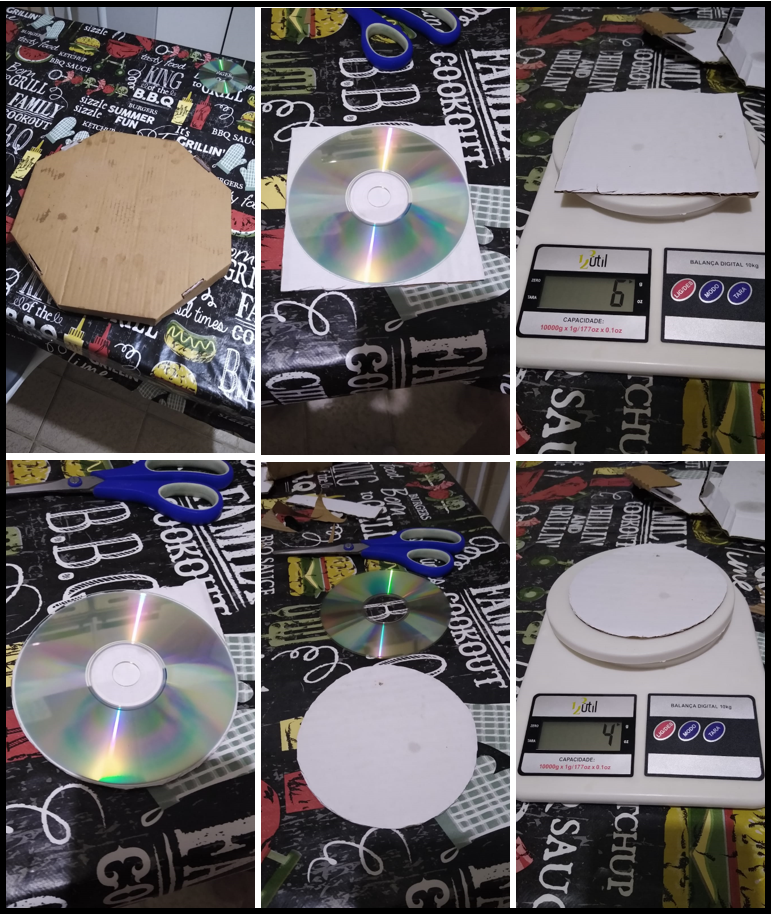
\includegraphics[width=0.7\linewidth]{PROGRAMACAO/pic/educacao/processo_01}
	\caption[]{Processo de construção dos objetos para a determinação da massa do quadrado e do círculo}
	\label{fig:processo01}
\end{figure}

Substituindo os valores na relação de $\pi$, tem-se:

\begin{ceqn}
	\begin{align*}
	\pi &= \frac{12 \cdot 12 \cdot 4}{6 \cdot 6^2} \\
	\pi &= \frac{144 \cdot 4}{216} \\
	\pi &= \frac{576}{216} \\
	\pi &= 2,666... \\
	\end{align*}
\end{ceqn}

Bom, claramente o valor que sabemmos sobre $\pi$ não é esse, mas \textit{onde está o erro?} A metodologia utilizada parece ser coerente e era de esperar uma diferença, pequena, mas poderia existir. Então, deve-se contentar com este resultado ou investigar mais? Obviamente que a investigação deve continuar e isso faz parte do processo; não basta apenas determinar uma metodologia e quando chegar no resultado final, OK, para! O resultado tem que ter SIGNIFICADO!

Uma possibilidade de investigação para ter um erro tão grande assim, está relacionada a \textit{precisão da balança}. 

Todo equipamento possui uma \textit{precisão}, ou seja, os equipamentos conseguem efetuar operações até um certo limite, após esse limite, os resultados não podem ser considerados.

A balança utilizada foi uma balança de cozinha que tem a capacidade de medir massas de até $10 kg$ com a unidade mínima em \textit{grama}, ou seja, ela consegue medir de 1 em 1 grama até 10 kg; Essa precisão não pode ser negligenciada dependendo do tamanho da massa que se mede, pois se medir algo que tenha 500 g, a forma correta de representação, nesse caso, seria $500 \pm 1 \text{g}$, sendo assim, esse objeto pode ter entre 499 e 501 grama. 

Os objetos do experimento possuem 6 g e 4 g, e através da balança utilizada, a medição pode ser 5-7 g e 3-5 g. Se dividir a precisão 1 g pela massa dos objetos tem-se: 0,17 ($\approx 16.7\%$) e 0,25 ($\approx 25 \%$), ou seja, a precisão da balança está na mesma \textit{Ordem de grandeza} da medida das massas dos objetos. Solução? Fazer mais quadrados e mais círculos com os mesmos tamanhos dos anteriores para que a precisão da balança fique em uma ordem de grandeza menor. As novas medições podem ser vistas na figura abaixo:

\begin{figure}[H]
	\centering
	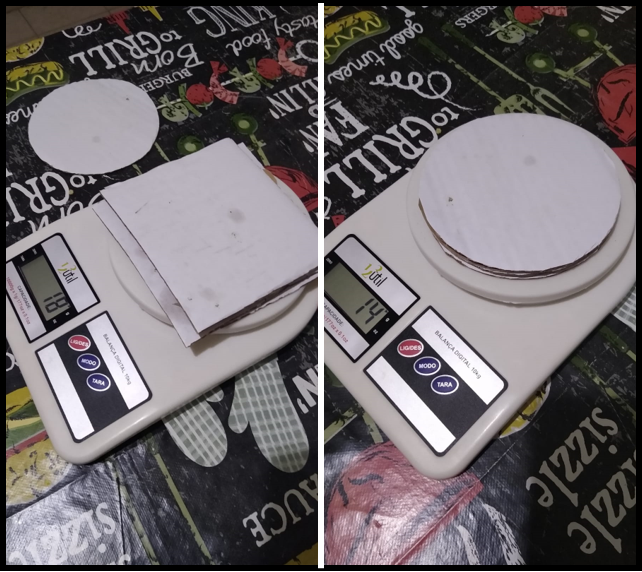
\includegraphics[width=0.7\linewidth]{PROGRAMACAO/pic/educacao/processo_02}
	\caption[]{Novas medições das massas.}
	\label{fig:processo02}
\end{figure}

Com essas novas medidas, a precisão da balança representa, apenas, $7,1\%$ da massa dos círculos e $5,6\%$ da massa dos quadrados. Assim, usando esses novos valores para as massas na relação montada para a determinação do $\pi$, tem-se:

\begin{ceqn}
	\begin{align*}
	\pi &= \frac{12 \cdot 12 \cdot 14}{18 \cdot 6^2} \\
	\pi &= \frac{144 \cdot 14}{18 \cdot 36} \\
	\pi &= \frac{2016}{648} \\
	\pi &= 3,111... \\
	\end{align*}
\end{ceqn}


Esse valor calculado representa muito bem o valor de $\pi$. O erro relacionado a este cálculo é de $0,9\%$. \textit{É possível melhorar o resultado?} Sim, é possível, usando uma balança de precisão, materiais de maior qualidade e homogêneos mas, para um processo de ensino-aprendizagem esse valor é surpreendente! Não pelo fato de ter calculado o valor aproximado, mas a quantidade de outros conhecimentos que podem ser discutidos.

\begin{exercise}
	Após a leitura desse texto, elabora um texto curto descrevendo o seu entendimento sobre Tecnologia.
\end{exercise}

\begin{exercise}
	A metodologia usada para a determinação do número $\pi$ experimentalmente possui uma quantidade de conhecimentos extras, ou seja, fora da exclusividade da matemática que podem ser explorados. Qual(is) desse(s) conhecimento(s) você nunca ouviu falar ou, foi extremamente diferente?
\end{exercise}

\begin{exercise}
	O tema do capítulo desse "futuro livro" está relacionado a \textit{softwares} mas, onde está a \textit{utilização do software}? Qual a relação desse tópico com a disciplina? 
\end{exercise}

\section{\textit{Softwares}}\index{\textit{Softwares}}

Muitos problemas na matemática podem ser resolvidos de \textit{modo analítico}, ou seja, sua solução pode ser calculada algebricamente, ou podem ser resolvidos de modo \textit{numérico}. Devido ao avanço da tecnologia, os computadores e, consequentemente, os \textit{softwares} permitem também cálculos algébricos.

Os matemáticos estão acostumados com algumas linguagens de programação e/ou softwares